\begin{section}{Resultados}

	Para analizar las diferencias y/o similitudes en la aplicación práctica de los tres algoritmos implementados se generaron gráficos que pasan a detallarse a continuación. 
		
	El primero de ellos consiste en gráficar el error relativo en función de la cantidad de iteraciones para cada uno de los algoritmos. Se utilizó precisión fija de 51 bits ya que por precondición la cantidad de dígitos de la mantisa debe ser menor a 52, es decir, con 51 dígitos minimizamos el error. Conseguimos la precisión deseada mediante truncamiento.
	El eje del gráfico que corresponde al $error\;relativo$ está en escala logarítmica para poder apreciar mejor los valores correspondientes dado que estos decrecen exponencialmente.

	\begin{figure}[H]
	  \centering
		\includegraphics[width=10cm,angle=-90]{graficos/comparacion_1a42it_51p.eps}
	  \caption{Comparación del error relativo de las tres series variando de 1 a 42 la cantidad de términos calculados con precisión de 51 bits en la mantisa.}
	  \label{fig:51p}
	\end{figure}
	
	\VSP
	
	Se anexan a continuación, tres gráficos correspondientes a cada una de series en los cuales se grafican cuatro curvas correspondientes al error relativo dado precisiones diferentes, variando la cantidad de iteraciones. Para cada uno de ellos la escala del eje $x$ toma distintos valores, esto sucede ya que dependiendo del algoritmo para el cálculo $\pi$ el error relativo graficado varía a partir en distintos valores.
	
	La idea inicial de estos gráficos es poder contestar la pregunta de si existe o no relación entre el error y la cantidad de iteraciones, así como en qué afecta el uso de distintas precisiones.
	
	Estos gráficos se muestra en el siguiente orden: Gregory, Ramanujan y Machin. Todos ellos se encuentran en escala logarítmica en el eje $y$

	\underline{Nota:} Para cada precisión utilizada, el error relativo calculado es contra un valor de $\pi$ exacto en los primeros $\lceil\log_2{t}\rceil$ dígitos (en base diez), seguidos de cero.

	\begin{figure}[H]
	  \centering
		\includegraphics[width=10cm,angle=-90]{graficos/gregory_1a1000it.eps}
	  \caption{Comparación del error relativo de la serie de Gregory utilizando diferentes precisiones, variando de 1 a 1000 la cantidad de iteraciones.}
	  \label{fig:gregory_1000it}
	\end{figure}
	
	\VSP

	\begin{figure}[H]
	  \centering
		\includegraphics[width=10cm,angle=-90]{graficos/ramanujan_1a42it.eps}
	  \caption{Comparación del error relativo de la serie de Ramanujan utilizando diferentes precisiones, variando de 1 a 42 la cantidad de iteraciones.}
	  \label{fig:ramanujan_42it}
	\end{figure}
	
	\VSP	

	\begin{figure}[H]
	  \centering
		\includegraphics[width=10cm,angle=-90]{graficos/machin_1a100it.eps}
	  \caption{Comparación del error relativo de la serie de Machin utilizando diferentes precisiones, variando de 1 a 100 la cantidad de iteraciones.}
	  \label{fig:machin_100it}
	\end{figure}
	
	Para un posterior análisis, se agrega utilizando el mismo origen de datos, un gráfico restringiendo la visualizacion a los primeros valores del ejes de coordenadas $x$ para la serie de Machin.
	
	\VSP	
	\begin{figure}[H]
	  \centering
		\includegraphics[width=10cm,angle=-90]{graficos/machin_1a8it.eps}
	  \caption{Comparación del error relativo de la serie de Machin utilizando diferentes precisiones, variando de 1 a 8 la cantidad de iteraciones.}
	  \label{fig:machin_8it}
	\end{figure}
	
	\VSP	

	Se realizaron además, experimentaciones sobre el error relativo en función de la cantidad de bits de precisión (variando este parámetro de 1 a 51). A continuación se detallan los resultados de estos experimientos.
	
	Se corrieron las pruebas hasta 42 iteraciones debido a que la serie de $Ramanujan$ es informativa hasta esa iteración (a partir de 43 iteraciones devuelve $nan$), es decir, el error relativo presentado corresponde al error cometido al calcular 42 términos de la serie.
	
	El gráfico se presenta bajo una escala logarítmica en $y$.
	
	\begin{figure}[H]
	  \centering
		\includegraphics[width=10cm,angle=-90]{graficos/comparacion_42it_1a51p.eps}
	  \caption{Comparación del error relativo de las tres series en el término 42 variando de 1 y 51 la cantidad de bits en la mantisa.}
	  \label{fig:42it}
	\end{figure}
	
	\VSP
	
	Consideramos que es pertinente mostrar un nuevo gráfico fijando la cantidad de iteraciones en un valor menor para verificar si existe alguna diferencia o no. Elegimos arbitrariamente correr las pruebas con 5 iteraciones.
	
	\begin{figure}[H]
	  \centering
		\includegraphics[width=10cm,angle=-90]{graficos/comparacion_5it_1a51p.eps}
	  \caption{Comparación del error relativo de las tres series en el término 5 variando de 1 y 51 la cantidad de bits en la mantisa.}
	  \label{fig:5it}
	\end{figure}
	
	\VSP
	
	Creímos conveniente además para analizar las diferencias variando las iteraciones, realizar tres gráficos (uno para cada serie) graficando en cada uno de ellos cuatro curvas las que corresponden a diferentes cantidad de iteraciones. Cada uno de los gráficos representan el error relativo cometido en función de la precisión del cálculo (variando este último de uno a cincuenta y uno).
	
	Utilizaremos estos gráficos para poder ver el cambio de precisión modifica el error producido o no. La visualización de varias curvas con distintas precisiones tiene como objeto analizar en qué afecta el aumento de este parámetro.
	
	Los gráficos poseen escala logarítmica en el eje $y$ y se presentan en el siguiente orden: Gregory, Ramanujan y Machin.
	
	\begin{figure}[H]
	  \centering
		\includegraphics[width=10cm,angle=-90]{graficos/gregory_1a51p.eps}
	  \caption{Comparación del error relativo de la serie de Gregory fijando diferentes cantidades de términos en cada curva variando de 1 y 51 la cantidad de bits en la mantisa.}
	  \label{fig:gregory_51p}
	\end{figure}
	
	\VSP
	
	\begin{figure}[H]
	  \centering
		\includegraphics[width=10cm,angle=-90]{graficos/ramanujan_1a51p.eps}
	  \caption{Comparación del error relativo de la serie de Ramanujan diferentes cantidades de términos en cada curva variando de 1 y 51 la cantidad de bits en la mantisa.}
	  \label{fig:ramanujan_51p}
	\end{figure}
	
	\VSP

	\begin{figure}[H]
	  \centering
		\includegraphics[width=10cm,angle=-90]{graficos/machin_1a51p.eps}
	  \caption{Comparación del error relativo de la serie de Machin diferentes cantidades de términos en cada curva variando de 1 y 51 la cantidad de bits en la mantisa.}
	  \label{fig:machin_51p}
	\end{figure}
	
	\VSP

	\underline{Nota:} Para hacer más simple el análisis de los gráficos, cada par de valores correspondientes a puntos consecutivos del eje $x$, se los unió mediante una recta, funcionalidad utilizada de GNUPLOT.
	
	El último gráfico corresponde al error relativo en función de la cantidad de dígitos, pero evaluando las cotas obtenidas en el análisis teórico con el error relativo de implementación.
	
	La información obtenida en este gráfico, nos ayudará a poder discernir cuál es la relación que existe entre estos dos mundos.
	
	\VSP
	
	\begin{figure}[H]
	  \centering
		\includegraphics[width=10cm,angle=-90]{graficos/cotas.eps}
	  \caption{Comparación del error relativo de las tres series y los errores teóricos en función de la cantidad de bits de mantisa.}
	  \label{fig:cotas}
	\end{figure}
\end{section}
